\documentclass[thesis=M,english]{FITthesis}[2012/06/26]

\usepackage[utf8]{inputenc}

\usepackage{graphicx}
\usepackage{tabularx}
\usepackage{booktabs}
\usepackage{csvsimple}
\usepackage{rotating}
\usepackage{subcaption}
\usepackage[usenames,dvipsnames]{xcolor}
\usepackage{blindtext}
\usepackage{dirtree}
\usepackage{pifont}
\usepackage{tikz}
\usepackage{listings}


\newcommand{\myblindtext}{\textcolor{Gray}{\blindtext}}
\newcommand{\myBlindtext}{\textcolor{Gray}{\Blindtext}}
\newcommand{\todo}[1]{\textcolor{red}{[[#1]]}}
\newcommand{\edit}[1]{\textcolor{blue}{#1}}
\newcommand{\yesMark}{\textcolor{Green}{\ding{51}}}
\newcommand{\noMark}{\textcolor{red}{\ding{55}}}
\newcommand{\nodewidth}{2.5cm}
\newcommand{\nodeheight}{0.6cm}

\definecolor{myOrange}{RGB}{255,204,0} % #ffcc00

\csvset{
  myTable/.style={separator=semicolon,head to column names,table head=\toprule #1 \\ \midrule,table foot=\bottomrule}
}

\usetikzlibrary{arrows.meta,calc,decorations.pathreplacing,fit,matrix,positioning}
\pgfdeclarelayer{bg}
\pgfsetlayers{bg,main}
\tikzset{
  >=stealth,
  font=\footnotesize,
  node distance=\nodeheight,
  rect/.style={draw,fill=myOrange,shape=rectangle,minimum width=\nodewidth,minimum height=\nodeheight,inner sep=1mm,text height=1.5ex,text depth=0.25ex},
  circle/.style={draw,fill=myOrange,shape=circle,minimum size=\nodeheight,inner sep=0},
  line/.style={draw,->,very thick,rounded corners},
  struct/.style={matrix,inner sep=0,column sep=-\pgflinewidth},
}




\department{Department of Computer Systems}
\title{Current development of authenticated encryption and its usage in TLS protocol}
\authorGN{Jan}
\authorFN{Žák}
\authorWithDegrees{Bc. Jan Žák}
\supervisor{prof. Ing. Róbert Lórencz, CSc.}
\acknowledgements{\todo{Acknowledgements}}
\abstractEN{\todo{Summarize the contents and contribution of your work in a few sentences in English language.}}
\abstractCS{\todo{V několika větách shrňte obsah a přínos této práce v českém jazyce.}}
\placeForDeclarationOfAuthenticity{Prague}
\declarationOfAuthenticityOption{4} % TODO
\keywordsCS{\todo{Replace with comma-separated list of keywords in Czech.}}
\keywordsEN{\todo{Replace with comma-separated list of keywords in English.}}


\begin{document}


\begin{introduction}

At its core, the Internet is built on top of IP and TCP protocols, which are used to package data into small packets for transport. As these packets travel across the world, they cross many computer systems in many countries. Because the core protocols don't provide any security by themselves, anyone with access to the communication links can gain full access to the data as well as change the traffic without detection.

Over the last years, the Internet has grown into a major platform for the world's communication. The Internet's trustworthiness has become critical to its success. If a person cannot trust that they are communicating with the party they intend, they won't give out their confidential data. If they cannot be assured that delivered information isn't modified in transit, they won't trust it as much.

The important properties of confidentiality, authentication and integrity are currently best provided on the Internet by the TLS protocol. The HTTP protocol implements it in its secure HTTPS variant, which means using \textit{"https://"} URLs. In the past, websites have deployed HTTPS rarely, often only when financial transactions take place.

More recently, however, it has become apparent that nearly all activity on the Internet can be considered sensitive. If a third party can modify content in transit, the power of the Internet can easily be turned against the user. For example, internet providers can "harmlessly" insert advertisements into websites. More hostile attacks include editing crucial information on the website, or injecting malware.

The TLS protocol does not dictate which cryptographic algorithms need to be used. Instead, TLS serves as a framework establishing and maintaining a secure comminucation channel suitable for sending sensitive messages, while new cryptographic algorithms can be implemented using a common interface.

Currently the TLS protocol uses a MAC-then-Encrypt generic composition to achieve both confidentiality and integrity goals. More recently, the idea of providing both confidentiality and integrity goals using a single cryptosystem has become accepted. In this concept, the combination of encryption and authentication algorithm is replaced by a single authenticated encryption algorithm, such as AES-GCM.

In 2013, CAESAR was announced. It is a worldwide cryptographic competition, focused on finding new methods of authenticated encryption, that offer advantages against commonly used AES-GCM and will be suitable for widespread adoption. Submitted algorithms will be publicly evaluated by committee of researchers in fields of cryptography and cryptoanalysis.



\end{introduction}

\chapter{Modern cryptography}

\section{Kerckhoffs' principle}
\label{toc/kerckhoffs-principle}

All crypto algorithms are preferred to be public. A well-known \textit{Kerckhoffs' principle} roughly says, that the security of the cryptosystem must depend only on the secrecy of the key, and not on the secrecy of the algorithm. They are very good reasons for this rule. Algorithms are hard to change. They are built into software or hardware, which can be difficult to upgrade. In real world, the same algorithm is used for a very long time. It is hard enough to keep the key secret, keeping the algorithm secret is far more difficult and expensive.

From past we know that it is very easy to make a small mistake and create cryptographic algorithm that is weak. If the algorithm is secret, nobody will find this fault until the attacker tries to break it. If the algorithm is kept secret, you shouldn't trust it. If the algorithm is public, researchers worldwide can participate in analyzing and improving the algorithm and its implementation.

While the cipher is publicly known, the secret key still needs to be exchanged via another communication method, which prevents Eve from reading it. Alice and Bob can meet in person to exchange the key or Alice can mail it via public post service. The key exchange problem is covered more detailed in \todo{ref it}.

\section{Encryption}
\label{toc/encryption}

Encryption is the original goal of cryptography. It is the process of encoding messages in such a way that only authorized parties can read it. Encryption does not of itself prevent interception, but denies the message content to the interceptor.

The generic use case is: Alice and Bob\footnote{Alice, Bob and Eve are placeholder names commonly used when discussing cryptography, to identify an archetypal role of participant. Alice is a sender, Bob is a receiver and Eve is an eavesdropper. For the first time these names were used in Ron Rivest's paper introducing RSA public key cryptosystem. \cite{rsa} Since then, a number of other names have entered cryptographic literature, such as Malory for malicious active attacker.} want to communicate with each other. However, communication channels are assumed not to be secure. Eve is eavesdropping on the channel. Any message that Alice sends to Bob is also received by Eve. (The same applies for messages sent from Bob to Alice, but it is the same problem and the same solution will work for Bob's messages, so we concentrate to Alice messages.) How can Alice and Bob communicate without learning everything? (\autoref{figure/encryption-problem}) \cite[p.~23]{ferguson2010cryptography}

To prevent Eve from understanding the conversation, Alice and Bob want to use encryption. They first need to agree on a set of \textit{encrypt} and \textit{decrypt} function $E, D$ as in \autoref{figure/encrypt-and-decrypt-functions} (a cipher) and a secret encryption \textit{key} $K_e$. Then they can use encryption in their communication channel in \autoref{figure/encryption}.

So Alice wants to send a \textit{plaintext} message $m$. She first encrypts it using the encrypt function $E(K_e, m)$ to get a \textit{ciphertext} message $c$. It can be sent over the communication channel, because only Alice and Bob know how to decrypt it. When Bob receives the ciphertext, he can decrypt it using the decrypt function $D(K_e, c)$ to get the original plaintext $m$ that Alice wanted to send to him.

Now Eve tries to listen to the message, but she receives only ciphertext message $c$. If we assume she doesn't know the encryption key $K_e$, she can't decrypt it.

Example algorithms: RC4, DES, AES

\begin{figure}
  \centering
  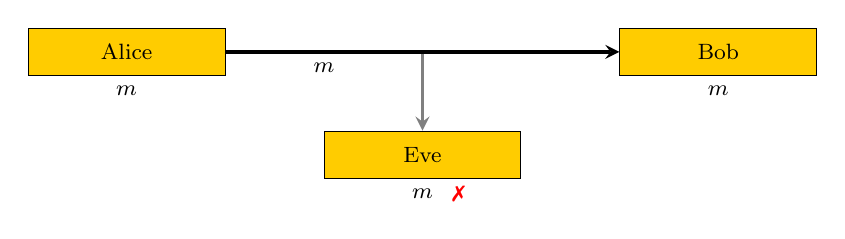
\begin{tikzpicture}
    \node (alice) [rect,left=2.5] {Alice};
    \node [below=0 of alice] {$m$};
    \node (bob) [rect,right=2.5] {Bob};
    \node [below=0 of bob] {$m$};
    \node (eve) [rect,below=1] {Eve};
    \node [below=0 of eve,label=right:{\noMark}] {$m$};
    \path [line,color=Gray] (0,0) -- (eve);
    \path [line] (alice) -- (bob) node[near start,below]{$m$};
  \end{tikzpicture}
  \caption{How can Alice and Bob communicate securely?}
  \label{figure/encryption-problem}
\end{figure}

\begin{figure}
  \centering
  \begin{subfigure}[b]{0.45\textwidth}
    \centering
    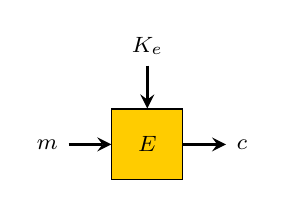
\begin{tikzpicture}
      \node (f) [rect,minimum size=1.5*\nodeheight] {$E$};
      \coordinate (k) at ($(f)+(0,1)$);
      \coordinate (m) at ($(f)-(1,0)$);
      \coordinate (c) at ($(f)+(1,0)$);
      \path [line,->] (k) -- (f) node[at start,above]{$K_e$};
      \path [line,->] (m) -- (f) node[at start,left]{$m$};
      \path [line,->] (f) -- (c) node[at end,right]{$c$};
    \end{tikzpicture}
    \caption{Encrypt function}
  \end{subfigure}
  \begin{subfigure}[b]{0.45\textwidth}
    \centering
    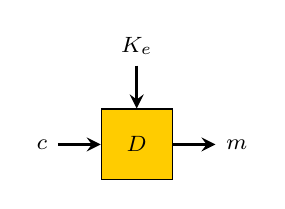
\begin{tikzpicture}
      \node (f) [rect,minimum size=1.5*\nodeheight] {$D$};
      \coordinate (k) at ($(f)+(0,1)$);
      \coordinate (c) at ($(f)-(1,0)$);
      \coordinate (m) at ($(f)+(1,0)$);
      \path [line,->] (k) -- (f) node[at start,above]{$K_e$};
      \path [line,->] (c) -- (f) node[at start,left]{$c$};
      \path [line,->] (f) -- (m) node[at end,right]{$m$};
    \end{tikzpicture}
    \caption{Decrypt function}
  \end{subfigure}
  \caption{Encrypt and decrypt function}
  \label{figure/encrypt-and-decrypt-functions}
\end{figure}

\begin{figure}[b]
  \centering

  \begin{subfigure}[b]{0.45\textwidth}
    \centering
    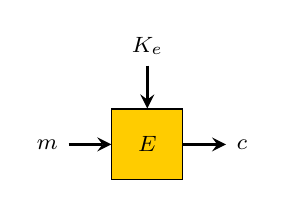
\begin{tikzpicture}
      \node (f) [rect,minimum size=1.5*\nodeheight] {$E$};
      \coordinate (k) at ($(f)+(0,1)$);
      \coordinate (m) at ($(f)-(1,0)$);
      \coordinate (c) at ($(f)+(1,0)$);
      \path [line,->] (k) -- (f) node[at start,above]{$K_e$};
      \path [line,->] (m) -- (f) node[at start,left]{$m$};
      \path [line,->] (f) -- (c) node[at end,right]{$c$};
    \end{tikzpicture}
    \caption{Encrypt function}
    \bigskip
  \end{subfigure}
  \begin{subfigure}[b]{0.45\textwidth}
    \centering
    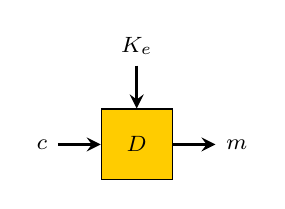
\begin{tikzpicture}
      \node (f) [rect,minimum size=1.5*\nodeheight] {$D$};
      \coordinate (k) at ($(f)+(0,1)$);
      \coordinate (c) at ($(f)-(1,0)$);
      \coordinate (m) at ($(f)+(1,0)$);
      \path [line,->] (k) -- (f) node[at start,above]{$K_e$};
      \path [line,->] (c) -- (f) node[at start,left]{$c$};
      \path [line,->] (f) -- (m) node[at end,right]{$m$};
    \end{tikzpicture}
    \caption{Decrypt function}
    \bigskip
  \end{subfigure}

  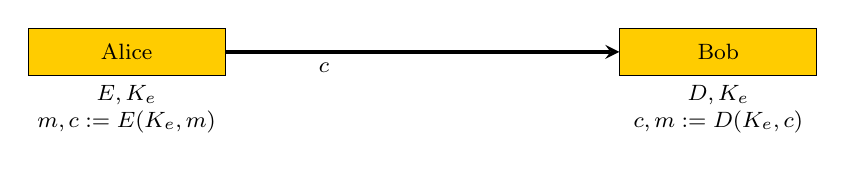
\begin{tikzpicture}
    \node (alice) [rect,left=2.5] {Alice};
    \node [align=center,below=0 of alice] {$E, K_e$ \\ $m, c := E(K_e, m)$};
    \node (bob) [rect,right=2.5] {Bob};
    \node [align=center,below=0 of bob] {$D, K_e$ \\ $c, m := D(K_e, c)$};
    \path [line] (alice) -- (bob) node[near start,below]{$c$};
  \end{tikzpicture}

  \caption{Generic setting for encryption}
  \label{figure/encryption}
\end{figure}


\section{Authentication}
\label{toc/authentication}

Alice and Bob have another problem, as shown in \autoref{figure/authentication-problem}. If Eve has a bit more control over the communication channel, she can not only passively listen to messages, she can also actively interfere.

To prevent Eve from undetectably modifying or forging messages, Alice and Bob want to use authentication. They first need to agree on a set of \textit{sign} and \textit{verify} functions $S, V$ as in \autoref{figure/sign-and-verify-functions} (usually the verify function simply uses the sign function and compares its results) and a authentication key $K_a$ (different from encryption key $K_e$). Then they can use authentication their communication channel in \autoref{figure/authentication}.

So Alice wants to send a message $m$. She first computes a signature $a$ using the sign function $S(K_a, m)$. This signature is also called Message Authentication Code (MAC). The message along with its signature can be sent over the communication channel, because only Alice and Bob know how to generate the signature. When Bob receives the message, he verifies the signature using the verify function $V(K_a, m, a)$, if it passes, he can be sure that Alice sent the message.

Now Eve tries to modify the message $m$ to a different message $m'$. If we assume that she doesn't know the authentication key $K_a$, she can only replace $m$ with $m'$. Bob will try to verify it, but it fails, so Bob will recognize that the message is not correct and he will discard it.

Pure authentication is only a partial solution. Eve can still do a lot of other malicious actions. Imagine Alice sending to Bob a messages containing requests for bank transfer. Eve can record a message and then send it to Bob later again (replay it), reorder messages, or completely delete messages. Therefore, authentication is almost always combined with a message numbering scheme. If a message $m$ contains such a message number, Bob is not fooled by Eve when she replays old messages. Bob will simply see that the message has correct signature, but the message number is from an old message, so he will discard it.

The best scheme of message numbering is a number sequence, incrementing by 1 for each message. Bob will accept only messages which passes the verification step and whose message number is strictly greater than the message number of the last message he accepted. So Bob receives a subsequence of messages of that Alice sent. A subsequence is simply the same sequence with growing message numbers with zero or more messages deleted.

Authentication with sequential message numbering solves most of the problem. Eve can still stop Alice and Bob from communicating by deleting or delaying messages. But that is all she can do. Alice and Bob can prevent the loss of information by using a scheme of resending messages that were lost, but that is more application-specific problem, and not part of cryptography.

Example algorithms: HMAC-MD5, HMAC-SHA1, HMAC-SHA256

\begin{figure}
  \centering
  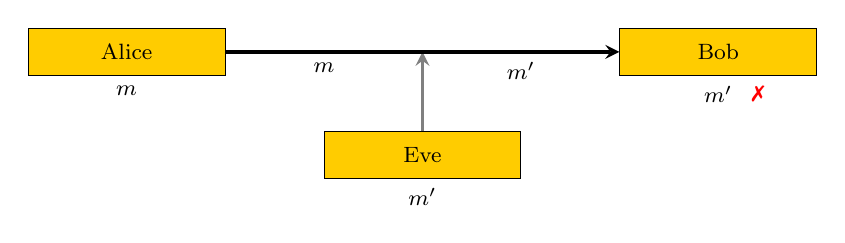
\begin{tikzpicture}
    \node (alice) [rect,left=2.5] {Alice};
    \node [below=0 of alice] {$m$};
    \node (bob) [rect,right=2.5] {Bob};
    \node [below=0 of bob,label=right:{\noMark}] {$m'$};
    \node (eve) [rect,below=1] {Eve};
    \node [below=0 of eve] {$m'$};
    \path [line,color=Gray] (eve) -- (0,0);
    \path [line] (alice) -- (bob) node[near start,below]{$m$} node[near end,below]{$m'$};
  \end{tikzpicture}
  \caption{How can Bob know who sent the message?}
  \label{figure/authentication-problem}
\end{figure}

\begin{figure}
  \centering
  \begin{subfigure}[b]{0.45\textwidth}
    \centering
    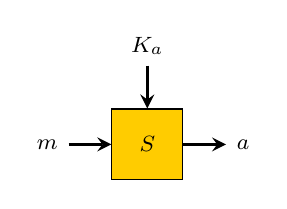
\begin{tikzpicture}
      \node (f) [rect,minimum size=1.5*\nodeheight] {$S$};
      \coordinate (k) at ($(f)+(0,1)$);
      \coordinate (m) at ($(f)-(1,0)$);
      \coordinate (a) at ($(f)+(1,0)$);
      \path [line,->] (k) -- (f) node[at start,above]{$K_a$};
      \path [line,->] (m) -- (f) node[at start,left]{$m$};
      \path [line,->] (f) -- (a) node[at end,right]{$a$};
    \end{tikzpicture}
    \caption{Sign function}
  \end{subfigure}
  \begin{subfigure}[b]{0.45\textwidth}
    \centering
    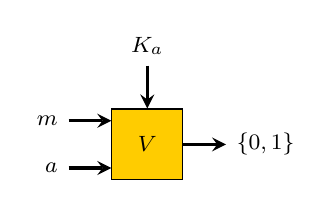
\begin{tikzpicture}
      \node (f) [rect,minimum size=1.5*\nodeheight] {$V$};
      \coordinate (k) at ($(f)+(0,1)$);
      \coordinate (m) at ($(f)-(1,0)$);
      \coordinate (a) at ($(f)-(1,0)$);
      \coordinate (r) at ($(f)+(1,0)$);
      \path [line,->] (k) -- (f) node[at start,above]{$K_a$};
      \path [line,->,transform canvas={yshift=0.5*\nodeheight}] (m) -- (f) node[at start,left]{$m$};
      \path [line,->,transform canvas={yshift=-0.5*\nodeheight}] (a) -- (f) node[at start,left]{$a$};
      \path [line,->] (f) -- (r) node[at end,right]{$\{0,1\}$};
    \end{tikzpicture}
    \caption{Verify function}
  \end{subfigure}
  \caption{Sign and verify functions}
  \label{figure/sign-and-verify-functions}
\end{figure}

\begin{figure}[b]
  \centering

  \begin{subfigure}[b]{0.45\textwidth}
    \centering
    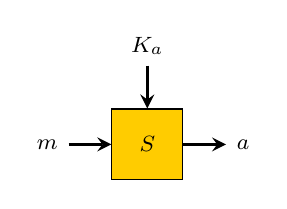
\begin{tikzpicture}
      \node (f) [rect,minimum size=1.5*\nodeheight] {$S$};
      \coordinate (k) at ($(f)+(0,1)$);
      \coordinate (m) at ($(f)-(1,0)$);
      \coordinate (a) at ($(f)+(1,0)$);
      \path [line,->] (k) -- (f) node[at start,above]{$K_a$};
      \path [line,->] (m) -- (f) node[at start,left]{$m$};
      \path [line,->] (f) -- (a) node[at end,right]{$a$};
    \end{tikzpicture}
    \caption{Sign function}
    \bigskip
  \end{subfigure}
  \begin{subfigure}[b]{0.45\textwidth}
    \centering
    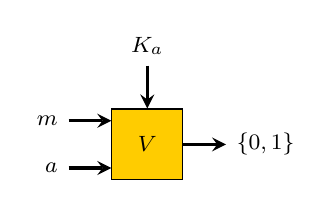
\begin{tikzpicture}
      \node (f) [rect,minimum size=1.5*\nodeheight] {$V$};
      \coordinate (k) at ($(f)+(0,1)$);
      \coordinate (m) at ($(f)-(1,0)$);
      \coordinate (a) at ($(f)-(1,0)$);
      \coordinate (r) at ($(f)+(1,0)$);
      \path [line,->] (k) -- (f) node[at start,above]{$K_a$};
      \path [line,->,transform canvas={yshift=0.5*\nodeheight}] (m) -- (f) node[at start,left]{$m$};
      \path [line,->,transform canvas={yshift=-0.5*\nodeheight}] (a) -- (f) node[at start,left]{$a$};
      \path [line,->] (f) -- (r) node[at end,right]{$\{0,1\}$};
    \end{tikzpicture}
    \caption{Verify function}
    \bigskip
  \end{subfigure}

  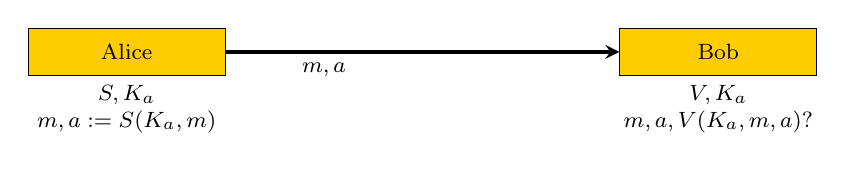
\begin{tikzpicture}
    \node (alice) [rect,left=2.5] {Alice};
    \node [align=center,below=0 of alice] {$S, K_a$ \\ $m, a := S(K_a, m)$};
    \node (bob) [rect,right=2.5] {Bob};
    \node [align=center,below=0 of bob] {$V, K_a$ \\ $m, a, V(K_a, m, a)?$};
    \path [line] (alice) -- (bob) node[near start,below]{$m, a$};
  \end{tikzpicture}

  \caption{Generic setting for authentication}
  \label{figure/authentication}
\end{figure}


\section{Asymmetric key exchange}

There is a huge disadvantage of encryption and authentication as discussed in \autoref{toc/encryption} and \autoref{toc/authentication}. Alice and Bob needs to share the key prior their communication starts, using a different, secure channel. Alice can't just sent the key to Bob over the same channel, as Eve could read it too.

Alice and Bob could have exchanged the key when they call themselves by a phone, or meet in person. Nevertheless, those channels can still be insecure or hard to maintain. It depends on Eve what capabilities to eavesdrop or modify them. In current modern age with pretty common high-budget surveilance, nobody can be sure about his digital privacy.

Distributing cryptographic keys is an old-age problem, and the solution lies in asymetric cryptography. It means that

By using a well-designed key exchange cryptosystem, Alice and Bob can establish a shared secret value, without sending it over an insecure channel. In short, they agree on common parameters, which they use for generating their secret values. Then they transform them to a public parameters, they exchange them, and using their own secret value, and the value from the opposite party, they can compute the shared secred value. If thecomputed value is kept secret, Alice and Bob can use it as a key for all crypto algorithms that needs a shared key. Eve can listen to key exchange parameters, but she can't compute the same value, because she doesn't know their secret exchange parameters.

\todo{example}

Example algorithms: Diffie-Hellman, ElGamal

\todo{image}

\section{Asymmetric encryption}

Asymmetric encryption can be also used for key exchange

\todo{text}

\autoref{figure/asymmetric-encryption}

\begin{figure}
  \centering
  \begin{subfigure}[b]{0.45\textwidth}
    \centering
    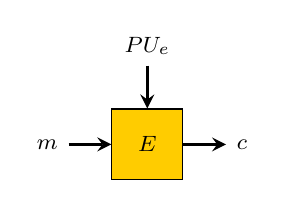
\begin{tikzpicture}
      \node (f) [rect,minimum size=1.5*\nodeheight] {$E$};
      \coordinate (k) at ($(f)+(0,1)$);
      \coordinate (m) at ($(f)-(1,0)$);
      \coordinate (c) at ($(f)+(1,0)$);
      \path [line,->] (k) -- (f) node[at start,above]{$PU_e$};
      \path [line,->] (m) -- (f) node[at start,left]{$m$};
      \path [line,->] (f) -- (c) node[at end,right]{$c$};
    \end{tikzpicture}
    \caption{Encrypt function}
  \end{subfigure}
  \begin{subfigure}[b]{0.45\textwidth}
    \centering
    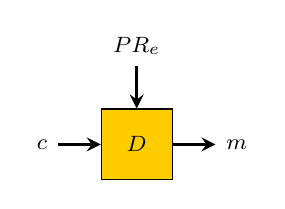
\begin{tikzpicture}
      \node (f) [rect,minimum size=1.5*\nodeheight] {$D$};
      \coordinate (k) at ($(f)+(0,1)$);
      \coordinate (c) at ($(f)-(1,0)$);
      \coordinate (m) at ($(f)+(1,0)$);
      \path [line,->] (k) -- (f) node[at start,above]{$PR_e$};
      \path [line,->] (c) -- (f) node[at start,left]{$c$};
      \path [line,->] (f) -- (m) node[at end,right]{$m$};
    \end{tikzpicture}
    \caption{Decrypt function}
  \end{subfigure}
  \caption{Asymmetric encrypt and decrypt functions}
\end{figure}

\begin{figure}
  \centering
  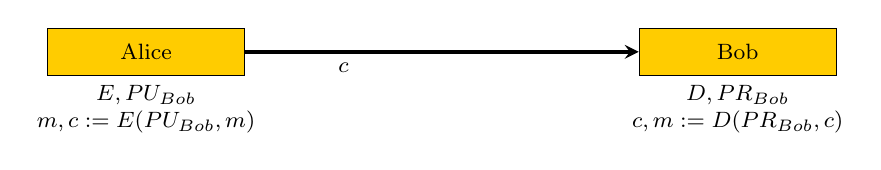
\begin{tikzpicture}
    \node (alice) [rect,left=2.5] {Alice};
    \node [align=center,below=0 of alice] {$E, PU_{Bob}$ \\ $m, c := E(PU_{Bob}, m)$};
    \node (bob) [rect,right=2.5] {Bob};
    \node [align=center,below=0 of bob] {$D, PR_{Bob}$ \\ $c, m := D(PR_{Bob}, c)$};
    \path [line] (alice) -- (bob) node[near start,below]{$c$};
  \end{tikzpicture}
  \caption{Generic setting for asymmetric encryption}
  \label{figure/symmetric-encryption}
\end{figure}


\section{Asymmetric authentication}

\todo{text}

\autoref{figure/asymmetric-authentication}

\begin{figure}
  \centering
  \begin{subfigure}[b]{0.45\textwidth}
    \centering
    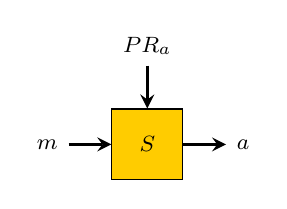
\begin{tikzpicture}
      \node (f) [rect,minimum size=1.5*\nodeheight] {$S$};
      \coordinate (k) at ($(f)+(0,1)$);
      \coordinate (m) at ($(f)-(1,0)$);
      \coordinate (a) at ($(f)+(1,0)$);
      \path [line,->] (k) -- (f) node[at start,above]{$PR_a$};
      \path [line,->] (m) -- (f) node[at start,left]{$m$};
      \path [line,->] (f) -- (a) node[at end,right]{$a$};
    \end{tikzpicture}
    \caption{Sign function}
  \end{subfigure}
  \begin{subfigure}[b]{0.45\textwidth}
    \centering
    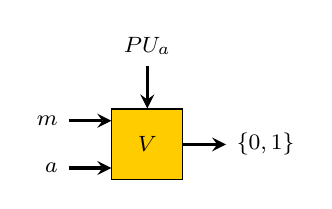
\begin{tikzpicture}
      \node (f) [rect,minimum size=1.5*\nodeheight] {$V$};
      \coordinate (k) at ($(f)+(0,1)$);
      \coordinate (m) at ($(f)-(1,0)$);
      \coordinate (a) at ($(f)-(1,0)$);
      \coordinate (r) at ($(f)+(1,0)$);
      \path [line,->] (k) -- (f) node[at start,above]{$PU_a$};
      \path [line,->,transform canvas={yshift=0.5*\nodeheight}] (m) -- (f) node[at start,left]{$m$};
      \path [line,->,transform canvas={yshift=-0.5*\nodeheight}] (a) -- (f) node[at start,left]{$a$};
      \path [line,->] (f) -- (r) node[at end,right]{$\{0,1\}$};
    \end{tikzpicture}
    \caption{Verify function}
  \end{subfigure}
  \caption{Asymmetric sign and verify functions}
\end{figure}

\begin{figure}
  \centering
  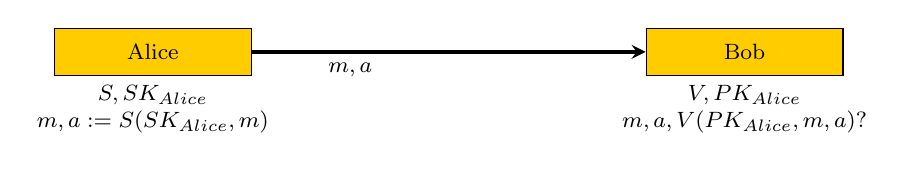
\begin{tikzpicture}
    \node (alice) [rect,left=2.5] {Alice};
    \node [align=center,below=0 of alice] {$S, SK_{Alice}$ \\ $m, a := S(SK_{Alice}, m)$};
    \node (bob) [rect,right=2.5] {Bob};
    \node [align=center,below=0 of bob] {$V, PK_{Alice}$ \\ $m, a, V(PK_{Alice}, m, a)?$};
    \path [line] (alice) -- (bob) node[near start,below]{$m, a$};
  \end{tikzpicture}
  \caption{Generic setting for asymmetric authentication}
  \label{figure/asymmetric-authentication}
\end{figure}


\section{Secure communication channel}

\todo{why symmetric encryption instead of asymmetric}

\todo{text}

\chapter{Authenticated Encryption}

\todo{popis AEAD}

\section{Block cipher modes}

from 70s

\begin{description}
  \item[ECB]
  \item[CBC]
  \item[CFB]
  \item[OFB]
  \item[CTR]
\end{description}

\todo{Block cipher modes image from @angealbertini}

Exploiting malleability:

ECB: Rearrange, replay blocks
CTR, OFB: Bitwise modification of blocks
CBC: Change current ciphertext block to predictably change the next plaintext block (during decryption)

Chosen-boundary attacks:

ECB, CBC, CFB: Partial chosen-plaintext control
Decrypt messages byte by byte

Here come the XOR ninjas

\section{Authenticated Encryption}
\section{Authenticated Encryption with Associated Data}



\section{Generic compositions}

\begin{description}
  \item[Encrypt-and-MAC]
  \item[MAC-then-Encrypt]
  \item[Encrypt-then-MAC]
\end{description}

\begin{figure}
  \centering
  \begin{subfigure}[b]{0.3\textwidth}
    \centering
    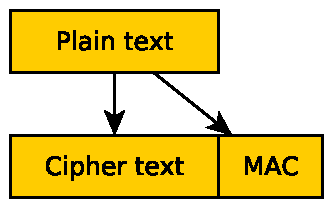
\includegraphics[width=0.9\textwidth]{images/encrypt-and-mac.pdf}
    \caption{Encrypt-and-MAC}
  \end{subfigure}
  \begin{subfigure}[b]{0.3\textwidth}
    \centering
    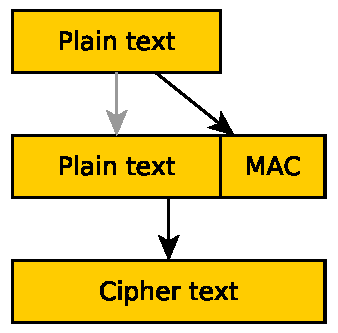
\includegraphics[width=0.9\textwidth]{images/mac-then-encrypt.pdf}
    \caption{MAC-then-encrypt}
  \end{subfigure}
  \begin{subfigure}[b]{0.3\textwidth}
    \centering
    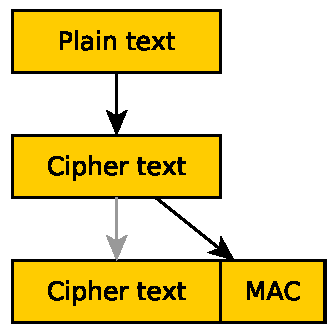
\includegraphics[width=0.9\textwidth]{images/encrypt-then-mac.pdf}
    \caption{Encrypt-then-MAC}
  \end{subfigure}
  \caption{Generic compositions of Authentized Encryption}
\end{figure}

\section{Competition for Authenticated Encryption: Security, Applicability and Robustness}

CAESAR is worldwide cryptographic competition, focused on finding new methods of authenticated encryption, that offer advantages against commonly used AES-GCM and will be suitable for widespread adoption. Submitted algorithms will be publicly evaluated by committee of researchers in fields of cryptography and cryptoanalysis.

\todo{popis algoritmů byly v soutěži, v čem se lišily, jaké a jak v nich byly nalezeny zranitelnosti a proto nepostoupily}

\todo{výběr algoritmu pro implementaci}

\subsection{Selection criteria}

\begin{description}
  \item[Online (one-pass)]
\end{description}



\subsection{NORX}

NO(T A)RX

ARX - Addition, Rotation, XOR

\subsubsection{Design goals}

\begin{itemize}
  \item \textbf{High security}
  \item \textbf{High speed} (in SW \textit{and} HW)
  \item \textbf{Simplicity} (of spec \textit{and} code)
  \item Online / one-pass
  \item Scalability (parallelism, unrolling)
  \item High key agility (no "key schedule")
  \item Side-channel leaks robustness (esp. timings)
\end{itemize}

\subsubsection{Parameters}

\begin{description}
  \item[Word Bit Size] $W \in {32, 64}$
  \item[Number of Rounds] $1 \leq R \leq 63$
  \item[Parallelism Degree] $0 \leq D \leq 255$ (0?)
  \item[Tag Bit Size] $|A| \leq 10W$
\end{description}

\begin{table}
  \centering
  \csvreader[
    after head=\begin{tabular}{llll}\toprule\csvlinetotablerow\\\midrule,
    late after line=\\,
    late after last line=\\\bottomrule\end{tabular}
  ]
    {tables/norx-proposed-instances.csv}{}
    {\texttt{\csvcoli} & \csvcolii & \csvcoliii & \csvcoliv}

  \caption{NORX proposed instances}
\end{table}

R=6: higher security margin

D=4: high throughput on parallel architectures

\subsection{Selection}

Benchmarks - Supercop, Brutus

\url{https://eprint.iacr.org/2014/850.pdf}
\url{http://www1.spms.ntu.edu.sg/~syllab/speed/}



\chapter{Competition for Authenticated Encryption: Security, Applicability and Robustness}

CAESAR is worldwide cryptographic competition, focused on finding new methods of authenticated encryption, that offer advantages against commonly used AES-GCM and will be suitable for widespread adoption. Submitted algorithms will be publicly evaluated by committee of researchers in fields of cryptography and cryptoanalysis.

\todo{popis algoritmů byly v soutěži, v čem se lišily, jaké a jak v nich byly nalezeny zranitelnosti a proto nepostoupily}

\todo{výběr algoritmu pro implementaci}

\section{Submission requirements}

An \textbf{authenticated cipher} is a function with five byte-string inputs and one byte-string output. The five inputs are:

\begin{description}
  \item[plaintext] variable-length
  \item[associated data] variable-length
  \item[secret message number] fixed-length
  \item[public message number] fixed-length
  \item[key] fixed-length
\end{description}

The first four inputs have different security purposes, as indicated by \autoref{table/caesar-inputs}.

\newcommand{\boldYes}[1]{%
  \ifthenelse{\equal{#1}{yes}}{\textbf{#1}}{#1}%
}

\begin{table}
  \centering
  \csvreader[
    after head=\begin{tabular}{lllll}\toprule\csvlinetotablerow\\\midrule,
    late after line=\\,
    late after last line=\\\bottomrule\end{tabular}
  ]
    {tables/caesar-inputs.csv}{}
    {\csvcoli & \boldYes{\csvcolii} & \boldYes{\csvcoliii} & \boldYes{\csvcoliv} & \boldYes{\csvcolv}}

  \caption{CAESAR inputs}
  \label{table/caesar-inputs}
\end{table}



The output is a variable-length ciphertext. The first four inputs have different security purposes, as indicated by the following table:

\section{C API}

\begin{lstlisting}
#define CRYPTO_KEYBYTES 16
#define CRYPTO_NSECBYTES 0
#define CRYPTO_NPUBBYTES 12
#define CRYPTO_ABYTES 16

#include "crypto_aead.h"

int crypto_aead_encrypt(
unsigned char *c,unsigned long long *clen,
const unsigned char *m,unsigned long long mlen,
const unsigned char *ad,unsigned long long adlen,
const unsigned char *nsec,
const unsigned char *npub,
const unsigned char *k
)
{
...
... the code for the cipher implementation goes here,
... generating a ciphertext c[0],c[1],...,c[*clen-1]
... from a plaintext m[0],m[1],...,m[mlen-1]
... and associated data ad[0],ad[1],...,ad[adlen-1]
... and secret message number nsec[0],nsec[1],...
... and public message number npub[0],npub[1],...
... and secret key k[0],k[1],...
...
return 0;
}

int crypto_aead_decrypt(
unsigned char *m,unsigned long long *mlen,
unsigned char *nsec,
const unsigned char *c,unsigned long long clen,
const unsigned char *ad,unsigned long long adlen,
const unsigned char *npub,
const unsigned char *k
)
{
...
... the code for the cipher implementation goes here,
... generating a plaintext m[0],m[1],...,m[*mlen-1]
... and secret message number nsec[0],nsec[1],...
... from a ciphertext c[0],c[1],...,c[clen-1]
... and associated data ad[0],ad[1],...,ad[adlen-1]
... and public message number npub[0],npub[1],...
... and secret key k[0],k[1],...
...
return 0;
}
\end{lstlisting}

npub - IV
nsec - nepoužito

\section{Submissions}

analyzovat každou podrobně je nad rámec této práce

the OCB mode, the GCM mode, the duplex sponge or AES-based block-cipher/permutation, Keccak-based permutation, stream-cipher based permutation

\section{Types}

\subsection{Duplex sponge functions}

Sponge as a design tool

On top of its original goal as a security reference, we realized that the sponge construction could also be used to build efficient cryptographic primitives. An important aspect is that the cryptographic primitive to be designed is a fixed-length permutation rather than harder-to-build structures such as block ciphers or dedicated compression functions. This is rather good news in itself, as all the symmetric cryptographic services can be realized using only a single primitive: a fixed-length permutation. As opposed to a block cipher, a fixed-length permutation makes no distinction between data and key input and hence can treat all input bits on an equal footing and at the same time can be made simpler.

\url{http://sponge.noekeon.org/}

The first 128-bit message block is handled directly, and taking in account the tag generation one needs m + 1 internal cipher calls to process messages of m block of n bits each. This is particularly important in many lightweight applications where message sent are usually composed of a few dozens of bytes (this is common disadvantage of sponge-based or stream cipher based lightweight designs like FIDES [2]) or ALE [8]).

Deoxys

Guido Bertoni, Joan Daemen, Michael Peeters, and Gilles Van Assche. Duplexing the Sponge: Single-Pass
Authenticated Encryption and Other Applications. In Ali Miri and Serge Vaudenay, editors, Selected Areas
in Cryptography, volume 7118 of LNCS, pages 320–337. Springer, 2011.

\subsection{Block modes}

It turns out that it is quite difficult to construct a secure lightweight authenticated cipher. Hence, it is meaningful to develop a secure lightweight authenticatedvencryption mode so that the previous designs of lightweight block ciphers can be converted to lightweight authenticated ciphers.

\section{Primitives}

AES

ARX - addition, rotation, XOR

LRX - logic, rotation, XOR

quaternions

\section{Selection criteria}

\subsection{Small messages}

It performs very well for small messages (only m + 1 calls to Joltik-BC are required for a m
block message and without any precomputation), in contrary to sponge or stream cipher based
lightweight designs that require a strong initialization stage. Such a feature is very important
as many constrained environments will only cipher very short messages (for example a 96-bit
Electronic Product Code)

Joltik

\begin{description}
  \item[Online (one-pass)]
\end{description}




\section{NORX}
\label{toc/caesar-norx}

NO(T A)RX

ARX - Addition, Rotation, XOR

\subsection{Design goals}

\begin{itemize}
  \item \textbf{High security}
  \item \textbf{High speed} (in SW \textit{and} HW)
  \item \textbf{Simplicity} (of spec \textit{and} code)
  \item Online / one-pass
  \item Scalability (parallelism, unrolling)
  \item High key agility (no "key schedule")
  \item Side-channel leaks robustness (esp. timings)
\end{itemize}

\subsection{Parameters}

\begin{description}
  \item[Word Bit Size] $W \in {32, 64}$
  \item[Number of Rounds] $1 \leq R \leq 63$
  \item[Parallelism Degree] $0 \leq D \leq 255$ (0?)
  \item[Tag Bit Size] $|A| \leq 10W$
\end{description}

\begin{table}
  \centering
  \csvreader[
    after head=\begin{tabular}{llll}\toprule\csvlinetotablerow\\\midrule,
    late after line=\\,
    late after last line=\\\bottomrule\end{tabular}
  ]
    {tables/norx-proposed-instances.csv}{}
    {\texttt{\csvcoli} & \csvcolii & \csvcoliii & \csvcoliv}

  \caption{NORX proposed instances}
\end{table}


R=6: higher security margin

D=4: high throughput on parallel architectures

\section{Selection}

Because the announcement of second-round candidates is in the time of writing this thesis still being postponed, I couldn't choose a well-rated candidate, which I would implement into OpenSSL. So I decided to implement a generic cipher using the CAESAR API (see \autoref{toc/caesar-api}).

As a reference cipher for my implementation part I chose NORX. It is not important which particular cipher I used, because the cipher can be easily switched for a different cipher complying with the CAESAR API, as soon as the the second-round candidate or final announcement will be made.


\chapter{Transport Layer Security (TLS) protocol}

\begin{figure}[t]
  \centering

  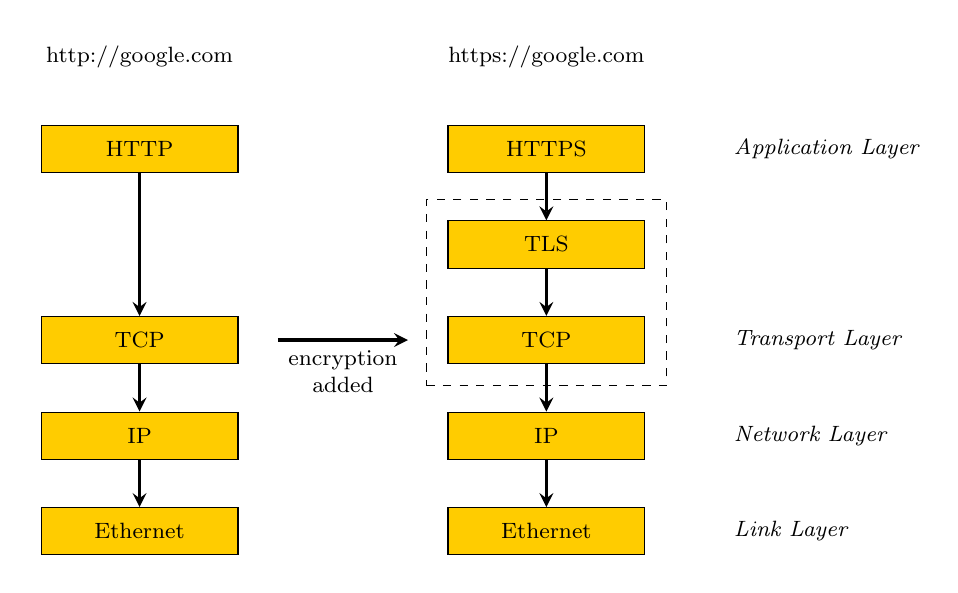
\begin{tikzpicture}
    \node (table) [matrix,row sep=\nodeheight,column sep=\nodewidth] {
      \node {\url{http://google.com}}; & \node {\url{https://google.com}}; \\
      \node (table-layer1) [rect] {HTTP}; & \node (table2-layer1) [rect] {HTTPS}; \\
      & \node (table2-layer2a) [rect] {TLS}; \\
      \node (table-layer2) [rect] {TCP}; & \node (table2-layer2b) [rect] {TCP}; \\
      \node (table-layer3) [rect] {IP}; & \node (table2-layer3) [rect] {IP}; \\
      \node (table-layer4) [rect] {Ethernet}; & \node (table2-layer4) [rect] {Ethernet}; \\
    };

    \node (table2-layer2) [draw,dashed,fit={($(table2-layer2a.north west)+(-0.25*\nodeheight,0.25*\nodeheight)$) ($(table2-layer2b.south east)+(0.25*\nodeheight,-0.25*\nodeheight)$)}] {};

    \node [right=1 of table2-layer1] {\textit{Application Layer}};
    \node [right=1 of table2-layer2b] {\textit{Transport Layer}};
    \node [right=1 of table2-layer3] {\textit{Network Layer}};
    \node [right=1 of table2-layer4] {\textit{Link Layer}};

    \path [line] (table-layer1) -- (table-layer2);
    \path [line] (table-layer2) -- (table-layer3);
    \path [line] (table-layer3) -- (table-layer4);

    \path [line] (table2-layer1) -- (table2-layer2a);
    \path [line] (table2-layer2a) -- (table2-layer2b);
    \path [line] (table2-layer2b) -- (table2-layer3);
    \path [line] (table2-layer3) -- (table2-layer4);

    \path [line,->] ($(table-layer2.east)+(0.5,0)$) -- ($(table2-layer2b.west)+(-0.5,0)$) node[midway,below,align=center] {encryption \\ added};
  \end{tikzpicture}

  \caption{Role of TLS in TCP/IP Reference Model}
  \label{figure/network-model}
\end{figure}


TLS is a security protocol used in almost 100\% of secure Internet transactions. Essentially, TLS transforms a typical reliable transport protocol (such as TCP) into a secure communication channel suitable for sending sensitive messages. TLS does not dictate which cryptographic algorithms need to be used. Instead, TLS serves as a framework establishing and maintaining a secure comminucation channel, while new cryptographic algorithms can be implemented using a common interface.

Adding encryption to an existing protocol is best performed in a transparent way, so that applications using the protocol library do not need to change their code to support encryption. A perfect example is HTTP protocol. A HTTP library can support both plaintext HTTP and encrypted HTTPS, and an application using this library can select the protocol simply in an URL, by specifying \textit{http://} or \textit{https://} respectively. See \autoref{figure/network-model}.

TLS has four main goals, listed here in the order of priority:

\begin{description}
  \item[Cryptographic security] This is the main issue: enable secure communication between any two parties who wish to exchange information.
  \item[Interoperability] Independent programmers should be able to develop programs and libraries that are able to communicate with one another using common cryptographic parameters.
  \item[Extensibility] TLS is effectively a framework for the development and deployment of cryptographic protocols. Its important goal is to be independent of the actual cryptographic primitives (e.g., ciphers and hashing functions) used, allowing migration from one primitive to another without needing to create new protocols.
  \item[Efficiency] The final goal is to achieve all of the previous goals at an acceptable performance costreducing costly cryptographic operations down to the minimum and providing a session caching scheme to avoid them on subsequent connections. \cite{ristic2014bulletproof}
\end{description}

Whereas TLS provides security over reliable TLS communication, there also exists its variant, DTLS protocol. DTLS is deliberately designed to be as similar to TLS as possible, both to minimize new security invention and to maximize the amount of code and infrastructure reuse. \cite{rfc6347} This thesis is about TLS only.

\section{Standardization}

The Internet is the result of a long-term collaboration between governments, academia, and businesses seeking to create a worldwide communication network. For the Internet to function correctly, it must be based upon standardized communication protocols.

Standards concerning the Internet are produced by the Internet Engineering Task Force (IETF) non-profit organization, where experts from around the world collaborates in work groups focused on specific area. IETF produces an informal series of documents known as Requests for Comments (RFCs). For a document to become an Internet standard, it is begins its life by being proposed as an RFC on the standardization track. RFCs in development are temporarily available as \textit{Internet Drafts}. After approval from IETF may be published as \textit{Proposed Standard}. \cite{dent2004user}

There are also other classes of RFCs, most notably experimental and informational RFCs. IETF RFCs cover all the topics of interest to an implementer working with the Internet, which would explain why there are so many of them\footnote{\url{http://www.rfc-editor.org/rfc-index.html}} - over 7400 at the time of writing.

Many of IETF RFCs describe security algorithms, protocols, or recommendations. The most interesting for this thesis are these produced by TLS working group\footnote{\url{https://tools.ietf.org/wg/tls/}}, such as:

\begin{description}
  \item[RFC2246] The TLS Protocol Version 1.0
  \item[RFC4346] The Transport Layer Security (TLS) Protocol Version 1.1
  \item[RFC5246] The Transport Layer Security (TLS) Protocol Version 1.2
  \item[draft-ietf-tls-tls13] The Transport Layer Security (TLS) Protocol Version 1.3 (work in progress)
  \item[RFC5288] AES Galois Counter Mode (GCM) Cipher Suites for TLS
  \item[RFC6655] AES-CCM Cipher Suites for Transport Layer Security (TLS)
\end{description}

TLS implementations are typically written as a set of functions that generate and parse all TLS record messages, and perform the relevant cryptographic operations. The state machine that this process must implement, is currently not standardized, and differs between implementations. Allowing unexpected transitions in this state machine can lead to unexpected behavior. There is an effort to standardize the TLS state machine to allow formal verification of core components in cryptographic protocol libraries. \cite{tls-state-machine}

\section{Records}

\begin{figure}
  \centering

  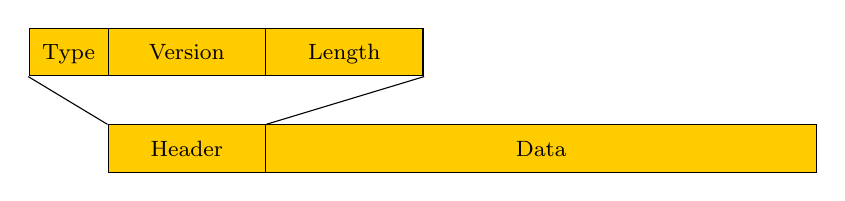
\begin{tikzpicture}
    \node (row1) [struct] {
      \node (type) [rect,minimum width=1cm] {Type}; & \node (version) [rect,minimum width=2cm] {Version}; & \node (length) [rect,minimum width=2cm] {Length}; \\
    };
    \node (row2) [struct,anchor=north west] at ($(row1.south west)+(1cm,-\nodeheight)$) {
      \node (header) [rect,minimum width=2cm] {Header}; & \node (data) [rect,minimum width=7cm] {Data}; \\
    };

    \path [draw] (row1.south west) -- (header.north west);
    \path [draw] (row1.south east) -- (header.north east);
  \end{tikzpicture}

  \caption{TLS record}
  \label{figure/tls-record}
\end{figure}


At a high level, TLS protocol specifies a structure of every record (packet). Each TLS record starts with a short header, which contains information about the record type (subprotocol), protocol version and data length. Message data follows the header. See \autoref{figure/tls-record} for record structure.

The record type is identified in the record by 1-byte integer ID as specified in \autoref{figure/tls-record-types}. The protocol version can be either SSL 3.0 (deprecated), TLS 1.0, TLS 1.1, TLS 1.2 and it is identified in the record by 2-byte integer ID as specified in \autoref{figure/tls-versions}. The data length field is 2-byte long and it specifies the message data length.

There are the following record types (subprotocols):

\begin{description}
  \item[Handshake protocol] The handshake protocol to negotiate connection parameters, such as the cipher suite, authenticate each other and verify that handhshake messages have not been modified by an attacker.
  \item[ChangeCipherSpec protocol] The ChangeCipherSpec protocol contains a single message, which is a signal from the sending side that it obtained enough information to generate the connection parameters, such as the encryption keys, and is switching all further communication to encryption. Client and server both send this message when the time is right.
  \item[Alert protocol] Alerts are intended to use a simple notification mechanism to inform the other side in the communication of exceptional circumstances. They're generally used for error messages, as listed in \autoref{figure/tls-alert-types}.
  \item[Application protocol] The Application protocol carries application messages, which are just opaque byte arrays as far as TLS is concerned. These messages are packaged, fragmented, and encrypted by the record layer, using the current connection security parameters, such as the negotiated cipher suite.
  \item[Heartbeat protocol] The Heartbeat protocol extension allows a keep-alive functionallity without performing renegotiation. Its purpose is intended especially for DTLS, however it is implemented also in TLS.
\end{description}

This thesis focuses on negotiation of the cipher suite in the Handshake protocol and on application data encryption in the Application protocol.

\section{Handshake protocol}
\label{toc/tls-handshake}

When a client and server start communicating, they use the handshake protocol to negotiate connection parameters, such as the cipher suite, authenticate each other and verify that handhshake messages haven't beed modified by an attacker. It is the most complex part of the TLS protocol, because it performs these tasks:

\begin{itemize}
  \item exchange supported capabilities and agree on shared connection parameters (TLS protocol version, cryptographic algorithms)
  \item exchange necessary cryptographic parameters to agree on shared secret values (\textit{master secret}) using public-key cryptography
  \item exchange certificates or other cryptographic information to authenticate one another
  \item verify that the handshake hasn't beed tampered by a third party
  \item verify that both parties have calculated the same secret values and they can be reliably used to transport application data via record protocol
\end{itemize}

This phase usually takes 6-13 messages (see \autoref{tls-handshake-types} for list of all message types) in 3-4 network flights, depending on which features are used. There can be many variations in the exchange, depending on the configuration and supported protocol extensions. In practice, we can see three common flows:

\begin{itemize}
  \item full handshake with client and server authentication
  \item basic handshake with server authentication
  \item abbreviated handshake that resumes an earlier session
\end{itemize}

\begin{figure}
  \centering

  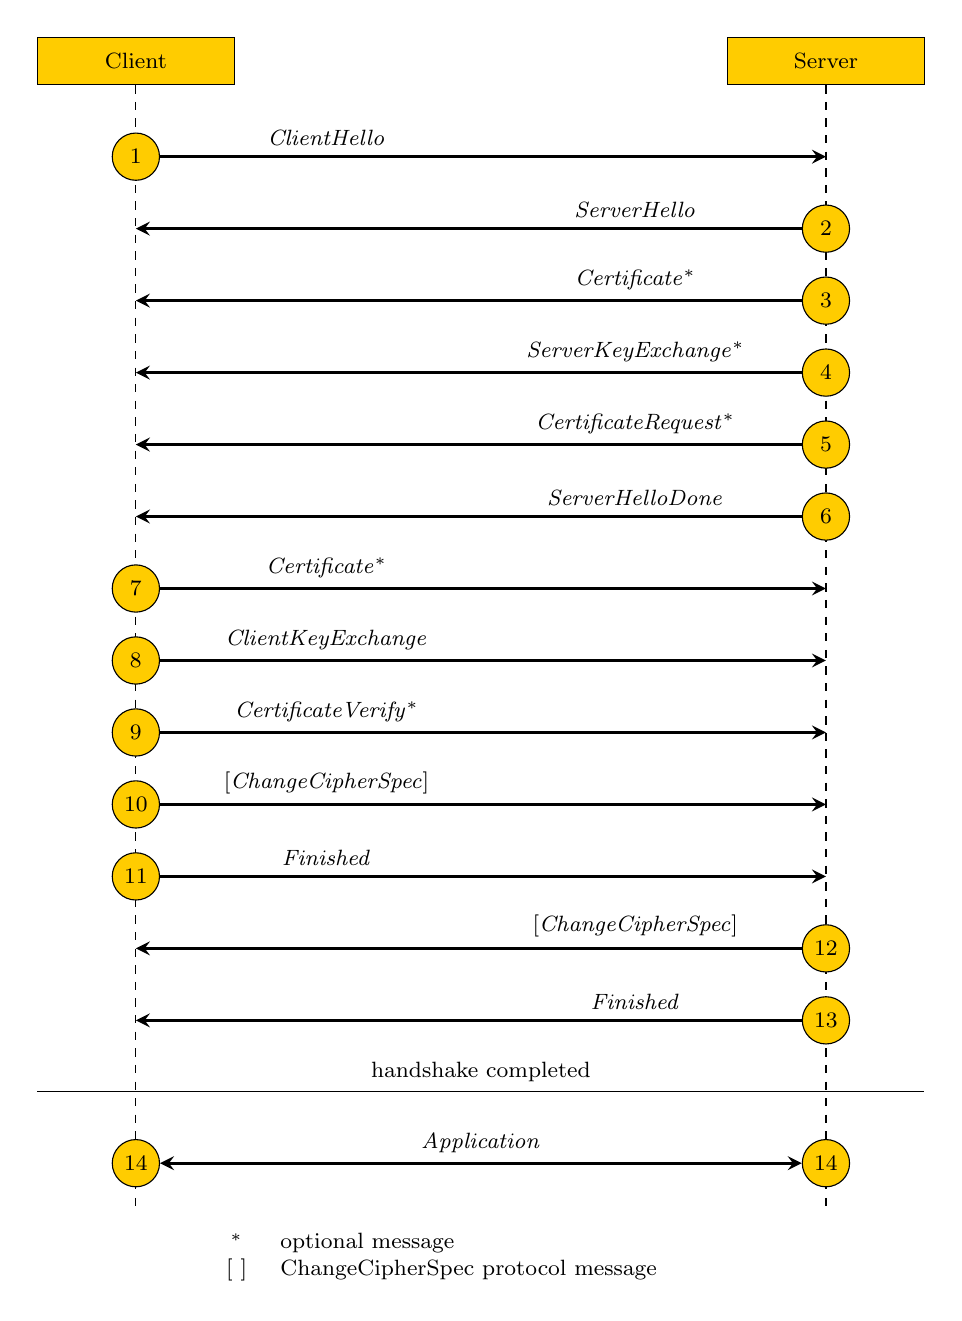
\begin{tikzpicture}
    \node (table) [matrix,row sep=0.5*\nodeheight,column sep=2.5*\nodewidth] {
      \node (client) [rect] {Client}; & \node (server) [rect] {Server}; \\[0.5*\nodeheight]
      \node (client1) [circle] {1}; & \coordinate (server1); \\
      \coordinate (client2); & \node (server2) [circle] {2}; \\
      \coordinate (client3); & \node (server3) [circle] {3}; \\
      \coordinate (client4); & \node (server4) [circle] {4}; \\
      \coordinate (client5); & \node (server5) [circle] {5}; \\
      \coordinate (client6); & \node (server6) [circle] {6}; \\
      \node (client7) [circle] {7}; & \coordinate (server7); \\
      \node (client8) [circle] {8}; & \coordinate (server8); \\
      \node (client9) [circle] {9}; & \coordinate (server9); \\
      \node (client10) [circle] {10}; & \coordinate (server10); \\
      \node (client11) [circle] {11}; & \coordinate (server11); \\
      \coordinate (client12); & \node (server12) [circle] {12}; \\
      \coordinate (client13); & \node (server13) [circle] {13}; \\[0.5*\nodeheight]
      \coordinate (client13b); & \coordinate (server13b); \\[0.5*\nodeheight]
      \node (client14) [circle] {14}; & \node (server14) [circle] {14}; \\
      \coordinate (client15); & \coordinate (server15); \\
    };

    \begin{pgfonlayer}{bg}
      \path [draw,dashed] (client) -- (client15);
      \path [draw,dashed] (server) -- (server15);
    \end{pgfonlayer}
    \path [line] (client1) -- (server1) node[above,near start] {\textit{ClientHello}};
    \path [line] (server2) -- (client2) node[above,near start] {\textit{ServerHello}};
    \path [line] (server3) -- (client3) node[above,near start] {\textit{Certificate}${}^\ast$};
    \path [line] (server4) -- (client4) node[above,near start] {\textit{ServerKeyExchange}${}^\ast$};
    \path [line] (server5) -- (client5) node[above,near start] {\textit{CertificateRequest}${}^\ast$};
    \path [line] (server6) -- (client6) node[above,near start] {\textit{ServerHelloDone}};
    \path [line] (client7) -- (server7) node[above,near start] {\textit{Certificate}${}^\ast$};
    \path [line] (client8) -- (server8) node[above,near start] {\textit{ClientKeyExchange}};
    \path [line] (client9) -- (server9) node[above,near start] {\textit{CertificateVerify}${}^\ast$};
    \path [line] (client10) -- (server10) node[above,near start] {[\textit{ChangeCipherSpec}]};
    \path [line] (client11) -- (server11) node[above,near start] {\textit{Finished}};
    \path [line] (server12) -- (client12) node[above,near start] {[\textit{ChangeCipherSpec}]};
    \path [line] (server13) -- (client13) node[above,near start] {\textit{Finished}};
    \path [draw] ($(client13b)-(0.5*\nodewidth,0)$) -- ($(server13b)+(0.5*\nodewidth,0)$) node[above,midway] {handshake completed};
    \path [line,<->] (client14) -- (server14) node[above,midway] {\textit{Application}};

    \node [below=0 of table,xshift=-5mm] {
      \begin{tabular}{cl}
        ${}^\ast$ & optional message \\
        $[$ $]$ & ChangeCipherSpec protocol message \\
      \end{tabular}
    };
  \end{tikzpicture}

  \caption{TLS full handshake}
  \label{figures/tls-full-handshake}
\end{figure}

\begin{figure}
  \centering

  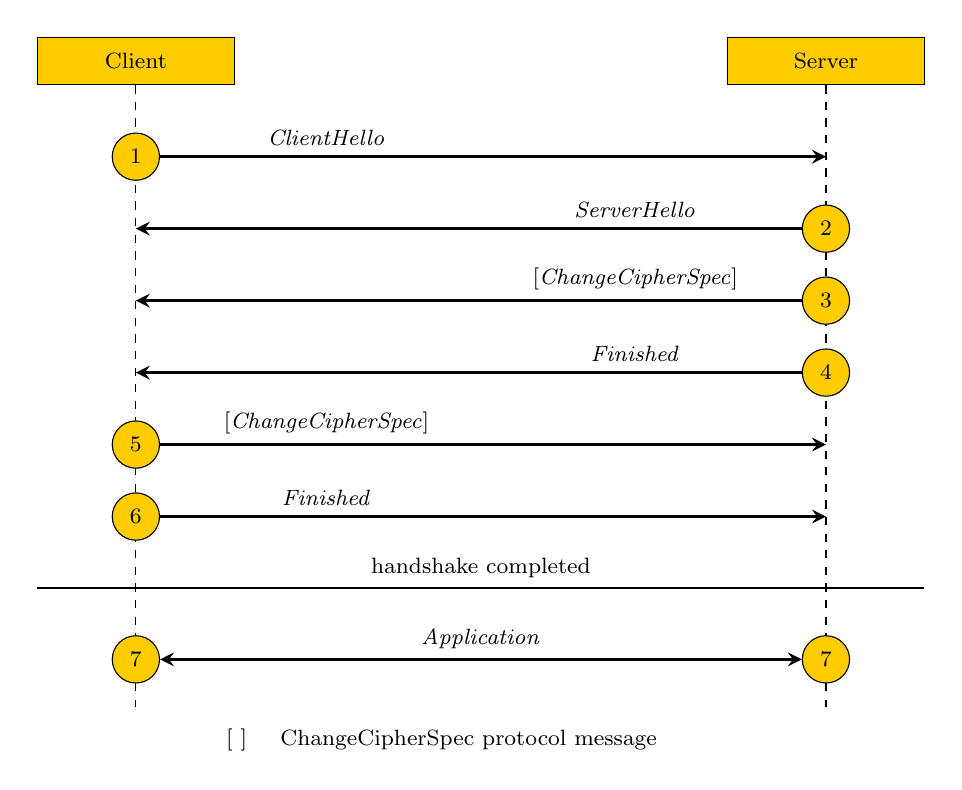
\begin{tikzpicture}
    \node (table) [matrix,row sep=0.5*\nodeheight,column sep=2.5*\nodewidth] {
      \node (client) [rect] {Client}; & \node (server) [rect] {Server}; \\[0.5*\nodeheight]
      \node (client1) [circle] {1}; & \coordinate (server1); \\
      \coordinate (client2); & \node (server2) [circle] {2}; \\
      \coordinate (client3); & \node (server3) [circle] {3}; \\
      \coordinate (client4); & \node (server4) [circle] {4}; \\
      \node (client5) [circle] {5}; & \coordinate (server5); \\
      \node (client6) [circle] {6}; & \coordinate (server6); \\[0.5*\nodeheight]
      \coordinate (client6b); & \coordinate (server6b); \\[0.5*\nodeheight]
      \node (client7) [circle] {7}; & \node (server7) [circle] {7}; \\
      \coordinate (client8); & \coordinate (server8); \\
    };

    \begin{pgfonlayer}{bg}
      \path [draw,dashed] (client) -- (client8);
      \path [draw,dashed] (server) -- (server8);
    \end{pgfonlayer}
    \path [line] (client1) -- (server1) node[above,near start] {\textit{ClientHello}};
    \path [line] (server2) -- (client2) node[above,near start] {\textit{ServerHello}};
    \path [line] (server3) -- (client3) node[above,near start] {[\textit{ChangeCipherSpec}]};
    \path [line] (server4) -- (client4) node[above,near start] {\textit{Finished}};
    \path [line] (client5) -- (server5) node[above,near start] {[\textit{ChangeCipherSpec}]};
    \path [line] (client6) -- (server6) node[above,near start] {\textit{Finished}};
    \path [draw] ($(client6b)-(0.5*\nodewidth,0)$) -- ($(server6b)+(0.5*\nodewidth,0)$) node[above,midway] {handshake completed};
    \path [line,<->] (client7) -- (server7) node[above,midway] {\textit{Application}};

    \node [below=0 of table,xshift=-5mm] {
      \begin{tabular}{cl}
        $[$ $]$ & ChangeCipherSpec protocol message \\
      \end{tabular}
    };
  \end{tikzpicture}

  \caption{TLS abbreviated handshake}
  \label{figures/tls-abbreviated-handshake}
\end{figure}


If a client and server hasn't previously communicated with each other, both parties will perform a full or basic handshake in order to establish a session. See \autoref{figures/tls-full-handshake}.

Full handshake requires client authentication, whereas basic handshake does not. Also it is possible to perform an anonymous handshake without any authentication, but it is not recommended, because it is sucpectible to MitM attacks.

A full handshake is completed after 4 network flights before the handshake is complete and protocol parties can begin to send application data. Thus, using TLS adds a latency penalty of 2 RTTs if the client sends application data first, such as in HTTP protocol.

\begin{enumerate}
  \item \textit{ClientHello} - client initiates a handshake, sends its capabilities to server
  \item \textit{ServerHello} - server selects the best connection parameters supported by both parties
  \item \textit{Certificate} - server sends its certificate chain (only if server authentication is required)
  \item \textit{ServerKeyExchange} - server sends additional information required to generate the master secret (only if it is required by selected cipher suite)
  \item \textit{CertificateRequest} - server requests client authentication and sends requirements for acceptable certificates (only if client authentication is required)
  \item \textit{ServerHelloDone} - server indicates completion of its side of negotiation
  \item \textit{Certificate} - client sends its certificate chain (only if client authentication is required)
  \item \textit{ClientKeyExchange} - client sends additional information required to generate the master secret
  \item \textit{CertificateVerify} - client proves the posession of private key corresponding to the previously sent client certificate (only if client authentication is required)
  \item \textit{ChangeCipherSpec} - client notifies server, that all following messages are encrypted
  \item \textit{Finished} - client sends a MAC of the handshake messages it sent and received
  \item \textit{ChangeCipherSpec} - server notifies client, that all following messages are encrypted
  \item \textit{Finished} - server sends a MAC of the handshake messages it sent and received
  \item handshake is completed, secure communication channel is established, both parties can securely send application data
\end{enumerate}

An abbreviated handshake is completed after 3 network flights, thus adding a latency penalty of just 1 RtT if the client sends application data first. See \autoref{figures/tls-abbreviated-handshake}. The session reuses previously exchanged secret values between the client and server, identified by either \textit{Session Tickets} or \textit{Session Cookies}.

\section{Cipher suites}

TLS is great in flexibility which provides for using various cryptographic primitives in a common framework. A selection of cryptographic primitives and their parameters is called \textit{cipher suite}.

A cipher suite is defined roughly by the following attributes:

\begin{itemize}
  \item Key exchange algorithm
  \item Authentication algorithm
  \item Encryption algorithm
  \begin{itemize}
    \item cipher algorithm
    \item key size
    \item cipher mode
  \end{itemize}
  \item MAC algorithm
  \item Pseudorandom function
\end{itemize}

Cipher suite names are usually long, descriptive and consistent. They are made from names of the key exchange method, authentiction method, encryption method and optional MAC or PRF algorithm.

\subsection{Key exchange}

\subsection{Authentication}

\subsection{Encryption}

\subsection{Message authentication}


\chapter{Implementing a new TLS cipher suite in OpenSSL}

\todo{popis částí v knihovně, které budu upravovat}

All cipher suites whose first byte is 0xFF are considered private and can be used for defining local/experimental algorithms. \cite[p.~55]{rfc2246}



\section{Creating new cipher}

\section{Creating new cipher suite}

\section{Testing}

\todo{compile a server and a client app with my edited library}
\todo{configure server to use the new cipher}
\todo{watch network traffic between them with Wireshark, confirm it is used}

All benchmarks were taken on a computer with the following configuration: CPU Intel Core i5-2540M (AES-NI, AVX capable), RAM 8 GB, OS Linux Fedora 21 (kernel 3.17.7, 64 bit).

openssl list-cipher-commands
openssl list-cipher-algorithms

openssl speed
generate cert
openssl s\_server -cert ...
openssl s\_client -connect 127.0.0.1:4433
openssl s\_time

\begin{conclusion}

  \todo{result}

\end{conclusion}

%\nocite{*}
\bibliographystyle{iso690}
\bibliography{DP_Zak_Jan_2015}

\appendix
\chapter{Acronyms}

\begin{description}
  \item[AEAD] Authenticated Encryption with Associated Data
  \item[AES] Anvanced Encryption Standard
  \item[AES-NI] Advanced Encryption Standard New Instructions
  \item[AVX] Advanced Vector Extensions
  \item[CAESAR] Competition for Authenticated Encryption: Security, Applicability and Robustness
  \item[DTLS] Datagram Transport Layer Security
  \item[IETF] Internet Engineering Task Force
  \item[ISO] International Organization for Standardization
  \item[LTS] Long Term Support
  \item[MAC] Message Authentication Code
  \item[PRF] Pseudorandom Function
  \item[RFC] Request for Comments
  \item[SSL] Secure Sockets Layer
  \item[TCP] Transmission Control Protocol
  \item[TLS] Transport Layer Security
  \item[UDP] User Datagram Protocol
\end{description}

\chapter{Content of attached CD}

\todo{obsah CD}

\begin{figure}
  \dirtree{%
    .1 readme.txt\DTcomment{the file with CD contents description}.
    .1 exe\DTcomment{the directory with executables}.
    .1 src\DTcomment{the directory of source codes}.
    .2 wbdcm\DTcomment{implementation sources}.
    .2 thesis\DTcomment{the directory of \LaTeX{} source codes of the thesis}.
    .1 text\DTcomment{the thesis text directory}.
    .2 thesis.pdf\DTcomment{the thesis text in PDF format}.
    .2 thesis.ps\DTcomment{the thesis text in PS format}.
  }
\end{figure}



\end{document}
